\documentclass[a4paper,10pt]{article}
\usepackage[utf8]{inputenc}
\usepackage[slovene]{babel}
\usepackage[left=2cm,top=2.3cm,right=2cm,nohead]{geometry}
\usepackage{amsmath}
\usepackage{amsfonts}
\usepackage{amssymb}
\usepackage[pdftex]{graphicx}
\usepackage{subfig}
\usepackage{textcomp}
\usepackage{tikz}
\usetikzlibrary{positioning,shapes,shadows,arrows,calc}

\begin{document}
\begin{titlepage}
  \let\footnotesize\small
  \let\footnoterule\relax
  \let \footnote \thanks
  \null\vfil
  \vskip 60pt
  \begin{center}
    {\LARGE \textbf{Hivemind} \\ Porazdeljeni Quake 2 bot \par}
    \vskip 3em
    {\large
     \lineskip .75em
      \begin{tabular}[t]{c}
        Grega Kešpret \\
        Jernej Kos \\
        Anže Vavpetič
      \end{tabular}\par}
      \vskip 1.5em
    {\large \today \par}
  \end{center}\par
  \vfil\null
\end{titlepage}


\section{Predstavitev in razdelitev problema}

\section{Pregled arhitekture rešitve}

% Shema arhitekture
\begin{center}
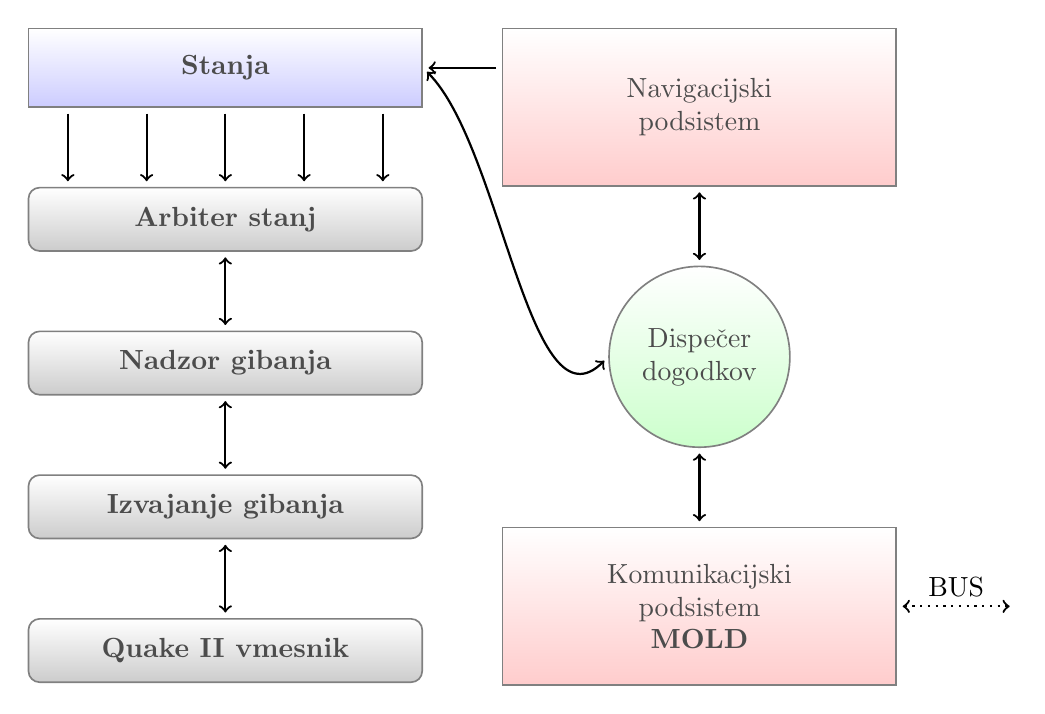
\begin{tikzpicture}[
  semithick,
	node distance=10mm,
	every node/.style={
		text centered
	},
	every path/.style={
		shorten >=2pt,
		shorten <=2pt,
		thick,
		arrows=-stealth'
	},
	colorednode/.style={
		color=black!70,
		rectangle,
		minimum height=6mm,
		minimum width=5cm,
		semithick,
		draw=black!50,
		top color=white,
		bottom color=black!20,
		rounded corners,
		inner sep=7pt
	},
	states/.style={
	  color=black!70,
		rectangle,
		minimum height=1cm,
		minimum width=5cm,
		semithick,
		draw=black!50,
		top color=white,
		bottom color=blue!20,
		inner sep=7pt
	},
	subsystem/.style={
	  color=black!70,
		rectangle,
		minimum height=2cm,
		minimum width=5cm,
		semithick,
		draw=black!50,
		top color=white,
		bottom color=red!20,
		inner sep=7pt
	},
	dispatcher/.style={
	  color=black!70,
		circle,
		minimum height=2cm,
		minimum width=2cm,
		semithick,
		draw=black!50,
		top color=white,
		bottom color=green!20,
		inner sep=7pt
	}
]

  \node (Q2Vmesnik) [colorednode] { \textbf{Quake II vmesnik} };
  \node (IzvajanjeGibanja) [colorednode, above=of Q2Vmesnik] { \textbf{Izvajanje gibanja} };
  \node (NadzorGibanja) [colorednode, above=of IzvajanjeGibanja] { \textbf{Nadzor gibanja} };
  \node (Arbiter) [colorednode, above=of NadzorGibanja] { \textbf{Arbiter stanj} };
  \node (Stanja) [states, above=of Arbiter] { \textbf{Stanja} };
  \node (Navigacija) [subsystem, right=of Stanja, yshift=-5mm] { \shortstack{ Navigacijski \\ podsistem } };
  \node (Dispatcher) [dispatcher, below=of Navigacija] { \shortstack{ Dispečer \\ dogodkov } };
  \node (Komunikacija) [subsystem, below=of Dispatcher] { \shortstack{ Komunikacijski \\ podsistem \\ \textbf{ MOLD } } };
  
  \draw[->] ($ (Stanja.south) - (2cm,0) $) -- ($ (Arbiter.north) - (2cm,0) $);
  \draw[->] ($ (Stanja.south) - (1cm,0) $) -- ($ (Arbiter.north) - (1cm,0) $);
  \draw[->] ($ (Stanja.south) - (0cm,0) $) -- ($ (Arbiter.north) - (0cm,0) $);
  \draw[->] ($ (Stanja.south) + (1cm,0) $) -- ($ (Arbiter.north) + (1cm,0) $);
  \draw[->] ($ (Stanja.south) + (2cm,0) $) -- ($ (Arbiter.north) + (2cm,0) $);
  \draw[<->] (Arbiter) -- (NadzorGibanja);
  \draw[<->] (NadzorGibanja) -- (IzvajanjeGibanja);
  \draw[<->] (IzvajanjeGibanja) -- (Q2Vmesnik);
  
  \draw[->] ($ (Navigacija.west) + (0,5mm) $) -- (Stanja);
  \draw[<->] (Navigacija) -- (Dispatcher);
  \draw[<->] (Dispatcher) -- (Komunikacija);
  \draw[<->] (Stanja.east) .. controls +(1,-1) and +(-1,-1) .. (Dispatcher.west);
  
  \draw[<->,dotted] (Komunikacija.east) -- node[above] {BUS} +(1.5cm,0); 
\end{tikzpicture}
\end{center}

\section{Vmesnik do virtualnega sveta}

\section{Nadzor gibanja in izogibanje oviram}

\subsection{Senzorji}

\subsection{Nadzorni sistem z EANN}

\subsection{Nadzorni sistem z mehko logiko}

\section{Navigacija po svetu}

\subsection{Statična geometrija iz BSP map}

\subsection{Samodejno učenje topografije}

\subsection{Iskanje poti skozi svet}

\section{Stanja robota}

\subsection{Arbitraža}

\subsection{Reinforcement learning}
% TODO a obstaja kakšen boljši slovenski izraz za RL?

\section{Komunikacija med instancami}

\subsection{MOLD (Message Oriented Lightweight Distributor)}

\subsection{Potek komunikacije}

\section{Možne izboljšave}

\section{Zaključek}

\end{document}

